\documentclass[../main.tex]{subfiles}

\begin{document}

Here we remark on a number of interesting patterns seen in our simulation: the curiously poor performance of the linear additive model, the relatively poor performance of the RBF models on the older-normal phenotype audiometric data, and the benefits of LSE over global acquisition functions for threshold estimation.

\subsection{Boundary over-exploration and the poor performance of linear-additive models}

The results above show consistently poor performance for the linear-additive model, even relative to previous reports. As noted above, part of this is driven by the use of variational inference over expectation propagation for inference. In addition, Song and colleagues report excluding the edges of the search space from model evaluation (but not from stimulus generation) ``due to known edge effects of PF estimation." We confirmed (simulations not shown) that evaluating only the interior of the audiometric test functions dramatically improves the performance of the additive-GP model while providing a marginal improvement at best to the full-RBF models, which brings the different model variants much closer to parity (though LSE acquisition still yields best performance).

These results demonstrate a key disadvantage of the linear kernel, in that it trades off between over-exploration and worse estimation of the latent slope. To see why, consider that the posterior covariance of any two points under the linear kernel is the product of their inputs. This means that posterior variance of $f$ will grow quadratically in the intensity dimension. This would generally not be a substantial problem because the probit function will squash very high and very low values to make the posterior variance in probability space small for very high or low probabilities. However, this is only possible if the latent function value can be allowed to go very large or small, which would worsen the estimate of the latent slope (and therefore position of the threshold and the function value itself). Without shrinking the posterior variance at values of the function far from the threshold, variance-sensitive acquisition functions like BALD and BALV will oversample in these areas of the space. Thus, the linear kernel creates an undesirable tradeoff between sampling irrelevant parts of the space and overestimating the slope of the latent psychometric function in the intensity dimension. This problem disappears with the use of the monotonic RBF kernel, which shows less boundary over-exploration than the linear kernel in spite of not using the over-exploration mitigation heuristic of Song and colleagues.

From a practical perspective, while we concur that boundary over-exploration in GPs is a known problem \citep[e.g.][]{Siivola2018}, it is not always practical to extend the search space to extreme stimulus values where thresholds are ignored---for example if these stimuli cannot be physically displayed by the hardware in question. As our objective is the practical usage of these methods across a breadth of psychophysical stimuli, the apparent robustness against boundary over-exploration is an additional benefit of our approach.

\subsection{Understanding the older-normal phenotype performance}

\begin{figure*}[!htb]
    \centering
    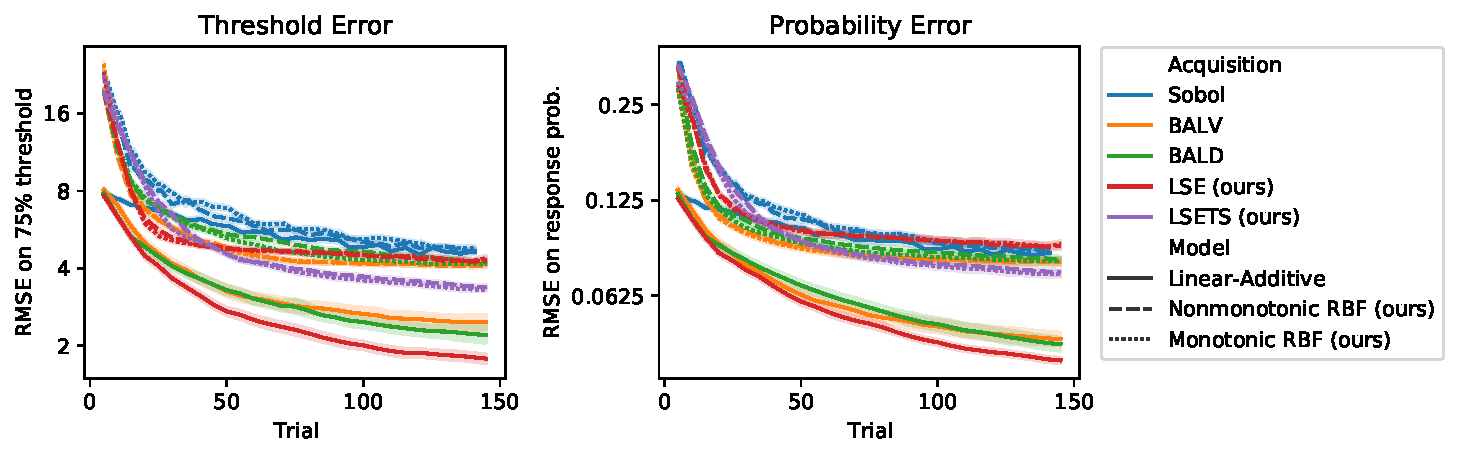
\includegraphics[width=\textwidth]{older-normal_pref.pdf}
    \caption{\textbf{Older-normal audiometric test function performance}. Performance is averaged over psychometric spread values. LSE is the best for acquisition in terms of error in both threshold (\emph{left}), and response probability (\emph{right}). The linear-additive model performs far better than the RBF models in this setting, and this performance gap exists from the beginning of sampling, consistent with the idea that this model's prior puts much more probability mass on this test function, which is relatively simpler. Shaded intervals are a 0.95 confidence interval over simulations.}
    \label{fig:song-older-normal}
\end{figure*}

The older-normal audiometric test function is the one case where the linear-additive model consistently performs best. Fig.~\ref{fig:song-older-normal} shows performance for this specific test function, averaged over psychometric spread values. It appears that with very limited data, the linear-additive model's prior is closer to the true threshold than the RBF models can achieve even with a much larger number of trials. Inspecting Fig.~\ref{fig:audiometric-thresholds} shows that in this phenotype the threshold is essentially flat as a function of frequency, and it would appear that the stronger prior of the linear-additive model allows it to capture that property much sooner. We see this as part of a broader pattern where simpler psychometric fields are more easily addressed by simpler models, and more complex ones (such as our novel discimination example) are better tackled with more flexible methods such as ours.

\section{Conclusion}

In this work, we have outlined a new nonlinear generalization of traditional psychophysics theory, where a stimulus-dependent Fechnarian relationship can yield rich nonlinear psychometric transfer functions. This generalized model, expressed as a Gaussian process (GP) with monotonicity information, allows for data-driven estimation of psychometric fields that respect theoretical constraints while remaining more flexible than either classical methods or other methods based on gaussian processes. To support this estimation, we have introduced to the field a new acquisition objective for adaptive psychometric testing targeting perceptual thresholds, the LSE. We have established the benefit of both contributions in extensive simulations, and have provided a software toolbox for application of these methods in real, human-subjects experiments.

\end{document}
